\appendix
\chapter{Network Generation Algorithm}
\begin{lstlisting}[language=Python]
def count_connections(n):
	if n == 1:
		return 0
	return count_connections(n-1)+n-1
		
def is_connection_in(c, cons):
	return c in cons or (c[1], c[0]) in cons
	
def random_pair(length):
	a = np.random.randint(0, length)
	b = a
	while b == a:
		b = np.random.randint(0, length)
	return a, b
	
def fully_connected_graph(nodes_names, density=0):
	# At 0 density the graph is connected minimally
	# (all nodes connect to all nodes)
	# At 1 density the graph is fully connected
	nodes = [[x] for x in nodes_names]
	# Make a random fully connected network
	connections = []
	while len(nodes) > 1:
		# Pick the two random groups
		# They cannot be the same group
		a, b = random_pair(len(nodes))
		na, nb = nodes[a], nodes[b]
		# Pick the member of each group to connect
		ma = na[np.random.randint(0, len(na))]
		mb = nb[np.random.randint(0, len(nb))]
		# Add a connection between them
		connections.append((ma, mb))
		
		# Make a new group that has all nodes
		# from the two groups that have been connected
		newgroup = []
		for n in na:
			newgroup.append(n)
		for n in nb:
			newgroup.append(n)
		nodes = [n for n in nodes
			if n not in [nodes[a], nodes[b]]]
		nodes.append(newgroup)
	# Add connections until we reach the density
	minimum_connections = len(connections)
	maximum_connections = count_connections(len(nodes_names))
	target_connections = 
		int((maximum_connections - minimum_connections)*density)
		+minimum_connections
	while len(connections) < target_connections:
		con = connections[0]
		while is_connection_in(con, connections):
			a, b = random_pair(len(nodes_names))
			con = (nodes_names[a], nodes_names[b])
		connections.append(con)
	return connections
\end{lstlisting}


\chapter{Machine Learning Model} \label{ap:model}
\begin{lstlisting}[language=Python]
inp = Input((28,28))
out = Reshape((28,28,1))(inp)
out = Conv2D(16, (3,3), activation="relu")(out)
out = Conv2D(16, (3,3), activation="relu")(out)
out = Flatten()(out)
out = Dense(256, activation="relu")(out)
out = Dense(128, activation="relu")(out)
out = Dense(10, activation="sigmoid")(out)
model = Model(inputs=inp, outputs=out)
model.compile(
	optimizer="adam",
	loss=SparseCategoricalCrossentropy(),
	metrics=[SparseCategoricalAccuracy()]
)
\end{lstlisting}

\chapter{Gantt Charts}
\newpage
\section{Gantt - Interim} \label{gc-interim}
\begin{center}
	\rotatebox[origin=c]{-90}{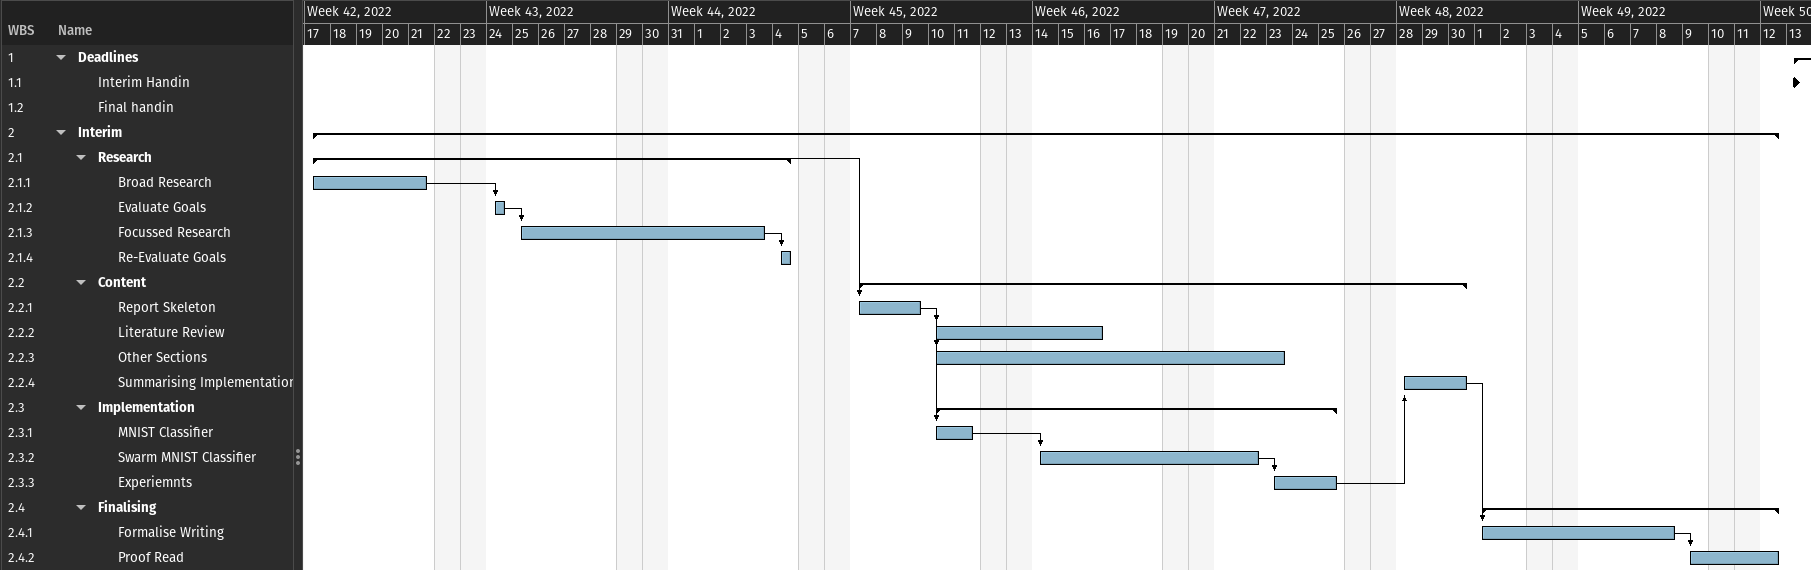
\includegraphics[width=\textheight]{gannt-interim}}
\end{center}

\section{Gantt - Final} \label{gc-final}
\begin{center}
	\rotatebox[origin=c]{-90}{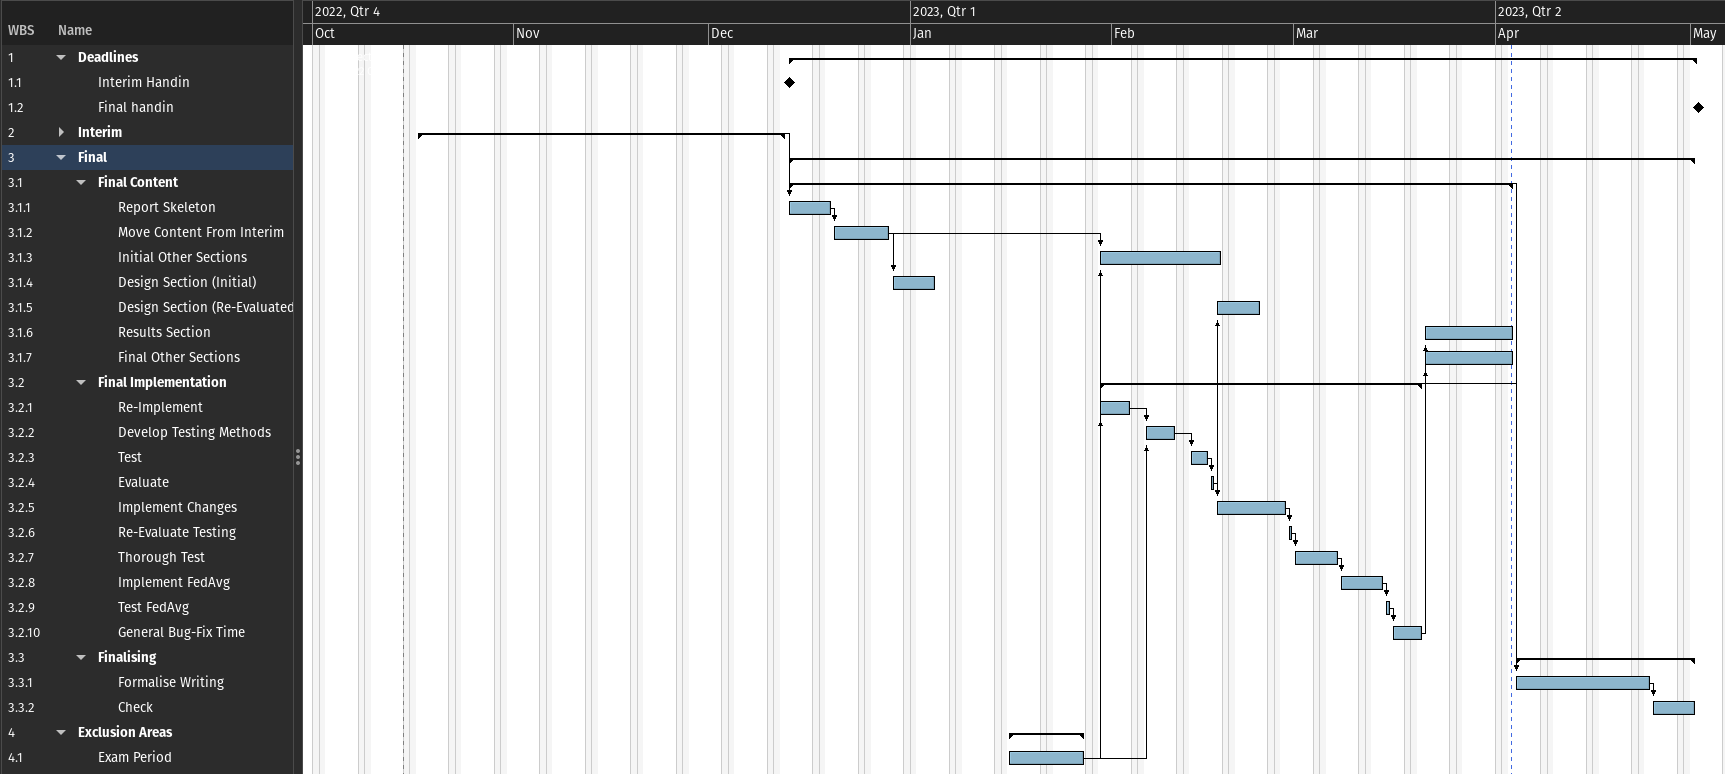
\includegraphics[width=\textheight]{gannt-final}}
\end{center}